%==============================================================================
%== template for LATEX poster =================================================
%==============================================================================
%
%--A0 beamer slide-------------------------------------------------------------
\documentclass[final]{beamer} % use beamer
\usepackage[orientation=portrait,
            size=a0,          % poster size
            scale=1.1         % font scale factor
           ]{beamerposter}    % beamer in poster size
%
%--some needed packages--------------------------------------------------------
\usepackage[american]{babel}  % language 
\usepackage[utf8]{inputenc}   % std linux encoding
\usepackage{caption}
\usepackage{subcaption}
% \usepackage[11pt]{moresize}
%
%==The poster style============================================================
\usetheme{cpbgposter}            % our poster style
%--set colors for blocks (without frame)---------------------------------------
  \setbeamercolor{block title}{fg=ngreen,bg=white}
  \setbeamercolor{block body}{fg=black,bg=white}
%--set colors for alerted blocks (with frame)----------------------------------
%--textcolor = fg, backgroundcolor = bg, dblue is the jacobs blue
  \setbeamercolor{block alerted title}{fg=white,bg=dblue!70}%frame color
  \setbeamercolor{block alerted body}{fg=black,bg=dblue!10}%body color
%
%==Titel, date and authors of the poster=======================================
\title{Finger formation at the base of ash clouds: \\ A linear stability analysis}
\author[shortname]{Paul Jarvis \inst{1} \and Jonathon Lemus \inst{1} \and
  Allan Fries \inst{1} \\ \and Amanda Clarke \inst{2} \and Jeremy Phillips \inst{3}
  \and Costanza Bonadonna \inst{1}}
\institute[shortinst]{\inst{1} Section of Earth and Environmental Sciences,
  University of Geneva \and
  \inst{2} School of Earth and Space Exploration, Arizona State University \and
  \inst{3} School of Earth Sciences, University of Bristol}

%
%==some usefull fluid dynamics====================================================
\newcommand\Rey{\mbox{\textit{Re}}}  % Reynolds number
\newcommand\Sc{\mbox{\textit{Sc}}}  % Schmidt number
%==============================================================================
%==the poster content==========================================================
%==============================================================================
\begin{document}
%--the poster is one beamer frame, so we have to start with:
\begin{frame}[t]

  \begin{columns}[t]

    \begin{column}{0.6\paperwidth}

      \begin{columns}[t]

        \begin{column}{0.3\paperwidth}

          \vspace{-2cm}

          \begin{figure}
            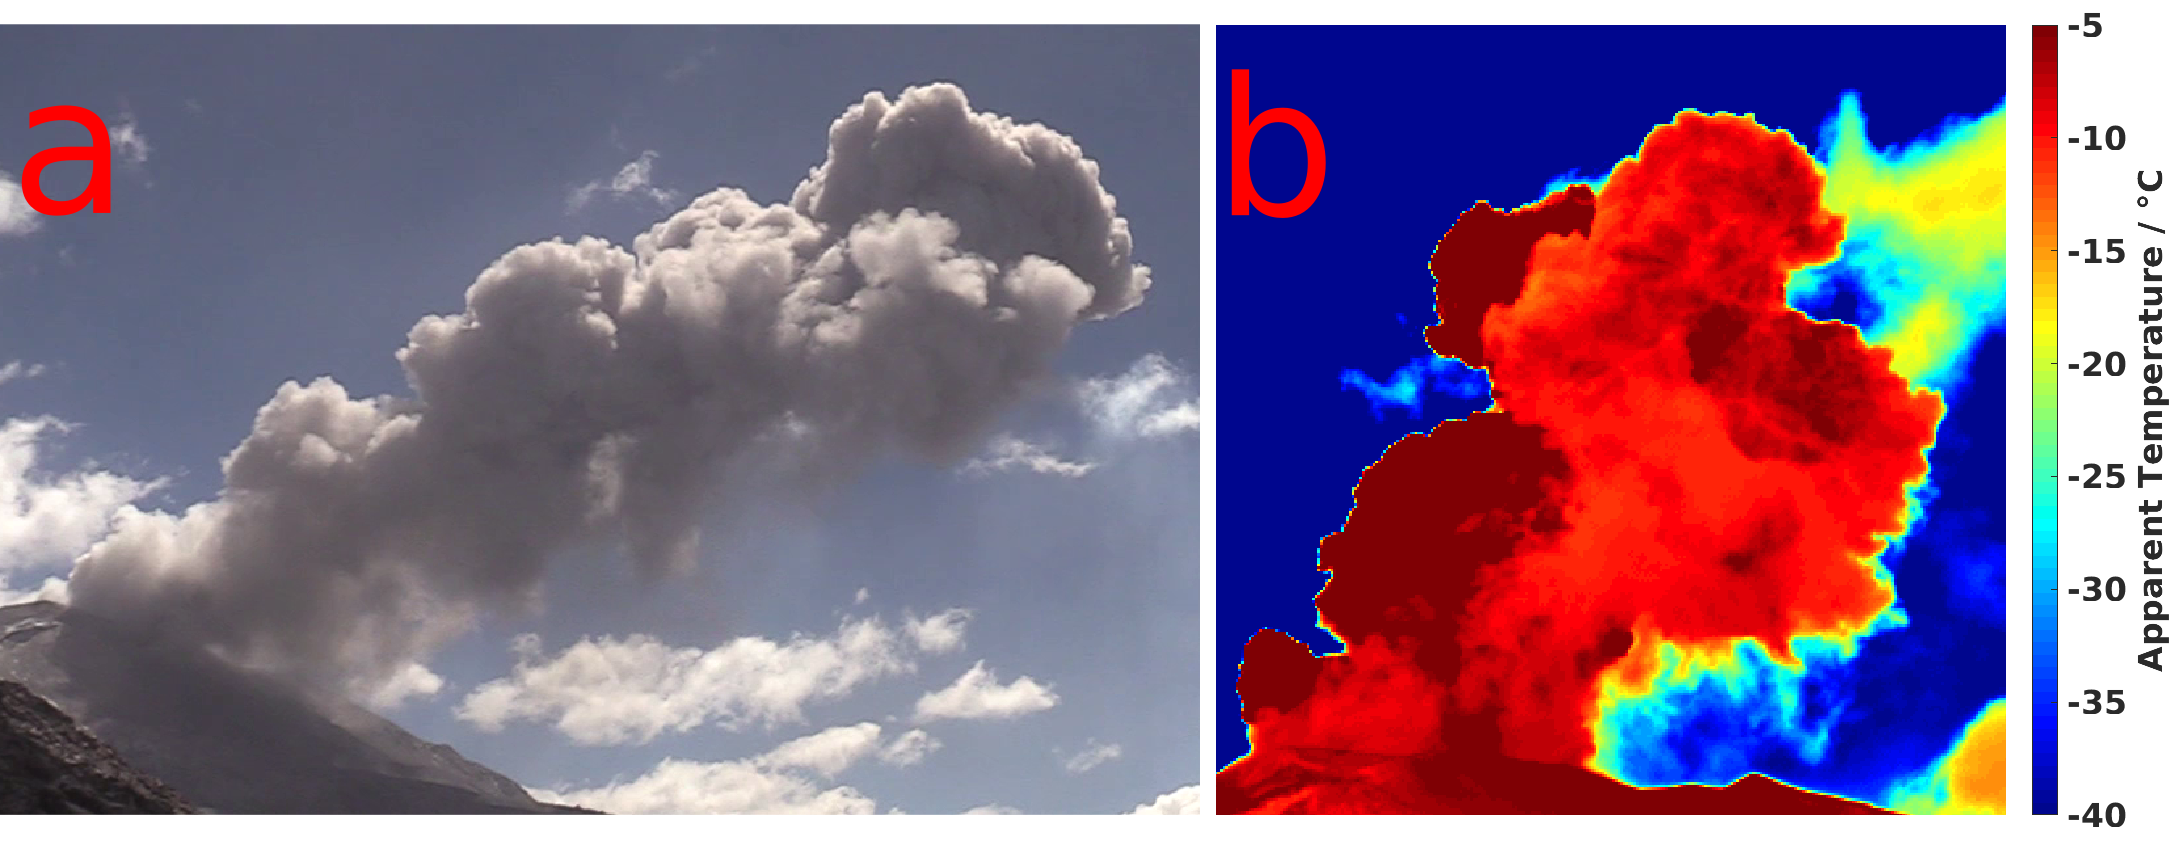
\includegraphics[width=\textwidth]{Sabancaya_fingers.png}
          \end{figure}

          \centering \footnotesize Figure 1. a) Visible and b) infrared images of
          ash clouds from Vulcanian explosions of Sabancaya volcano, Peru. Fingers
          can be seen in both images.

        \end{column}

        \begin{column}{0.3\paperwidth}

          \vspace{-2cm}

          \begin{block}{Introduction}

            \centering Volcanic ash presents a hazard for infrastructure and human
            health. Understanding ash settling is therefore crucial for assessing
            the associated risk. Downard-propagating fingers(Figure 1), hypothesised
            to form from a gravitational instability at the base of the ash cloud
            (Figure 2) have been seen at many volcanoes, and in analogue experiments
            (\textbf{Allan Fries}) and numerical models (\textbf{Jonathon Lemus}).
            Here we present a linear stability analysis, that predicits the initial
            growth rate of the fingers. 
          \end{block}

        \end{column}
      \end{columns}

      \begin{columns}[t]
        \begin{column}{0.43\paperwidth}

          \begin{block}{Equations of motion}

            \begin{columns}[t]

              \begin{column}{0.13\paperwidth}

                \centering

                Conservation of mass \\

                \vspace{1.75cm}

                Conservation of momentum \\

                \vspace{1.75cm}

                Conservation of particles \\

                \vspace{1.75cm}

                Conservation of solute \\

                \vspace{1.75cm}

                Reduced gravity 

              \end{column}

              \begin{column}{0.3\paperwidth}
                $$ \mathbf{\nabla} \cdot \mathbf{u}(\mathbf{x}, t) $$

                $$ \frac{\partial \mathbf{u}(\mathbf{x}, t)}{\partial t} +
                [\mathbf{u}(\mathbf{x}, t)] \cdot \mathbf{\nabla}]
                  \mathbf{u}(\mathbf{x}, t) =
                  \frac{\mathbf{\nabla} P(\mathbf{x}, t)}{\rho_{0}} +
                  \nu \nabla^{2} \mathbf{u}(\mathbf{x}, t) - g'\mathbf{\hat{z}} $$

                  $$ \frac{\partial \phi(\mathbf{x}, t)}{\partial t} +
                  [\mathbf{u}(\mathbf{x}, t)] - \mathbf{U_{\text{p}}}] \cdot
                    \mathbf{\nabla} \phi(\mathbf{x}, t) =
                    D_{\text{p}} \nabla^{2} \phi(\mathbf{x}, t) $$
                    
                    $$ \frac{\partial s(\mathbf{x}, t)}{\partial t} +
                    \mathbf{u}(\mathbf{x}, t)x \cdot \mathbf{\nabla} s(\mathbf{x}, t) =
                    D_{\text{s}} \nabla^{2} s(\mathbf{x}, t) $$

                    $$ g' = g \left(1 + \alpha s(\mathbf{x}, t) 
                    + \frac{\rho_{p} \phi(\mathbf{x}, t)}{\rho_{0}} \right) $$

              \end{column}

            \end{columns}
          \end{block}
        \end{column}
        \begin{column}{0.17\paperwidth}
          \begin{block}{Expansion}
            $$ \mathbf{u}(\mathbf{x}, t) = \mathbf{\hat{u}}(z) e^{i(k_{x} x + k_{y} y - \omega t)}$$

            $$ P(\mathbf{x}, t) = P^{(0)}(\mathbf{x}, t) +
            \hat{P}(z) e^{i(k x - \omega t)}$$

            $$ \phi(\mathbf{x}, t) = \phi^{(0)}(\mathbf{x}, t) +
            \hat{\phi}(z) e^{i(k x - \omega t)}$$
      
            $$ s(\mathbf{x}, t) = s^{(0)}(\mathbf{x}, t) +
            \hat{s}(z) e^{i(k x - \omega t)}$$

            $$\hat{P} \ll P^{(0)}, \hat{\phi} \ll \phi^{(0)}, \hat{s} \ll s^{(0)}$$
          \end{block}

        \end{column}
      \end{columns}
      
    \end{column}

    \begin{column}{0.3\paperwidth}

      \vspace{-3cm}
      
      \begin{columns}[t]
        \begin{column}{0.12\paperwidth}

          \vspace{-2.2cm}

          \begin{figure}
            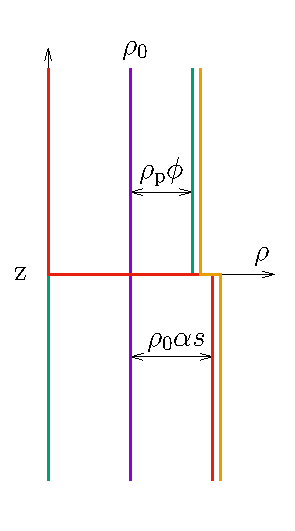
\includegraphics[height=20cm]{init_config.pdf}
          \end{figure}
        \end{column}

        \begin{column}{0.17\paperwidth}
          
          \begin{figure}
            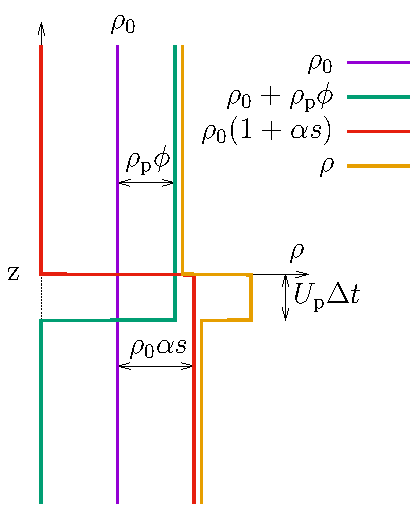
\includegraphics[height=18cm]{unstable_config.pdf}
          \end{figure}
        \end{column}
        
      \end{columns}

      \vspace{-1cm}

      \centering \footnotesize Figure 2. Despite an initial stable
      configuration, ash settling leads to the formation of a gravitationally
      unstable \textbf{particle boundary layer}.

      \vspace{1cm}

      \normalsize

      \begin{tabular}{| c | l | c | l |}
        \hline
        \multicolumn{2}{ | c |}{\textbf{Unknowns}}             & \multicolumn{2}{| c |}{\textbf{Parameters}}\\
        \hline
        $\mathbf{u}(\mathbf{x}, t)$ & Fluid velocity           & $\rho_{0} $           & Reference fluid density \\
        $P(\mathbf{x}, t)$          & Pressure                 & $\nu$                & Kinematic viscosity \\
        $\phi(\mathbf{x}, t)$       & Particle volume          &$\mathbf{U_{\text{p}}}$ & Particle settling velocity \\
        $s(\mathbf{x}, t)$          & Solute concentration     & $\rho_{\text{p}}$      & Particle density \\
        \cline{1-2}
        \multicolumn{2}{ | c |}{\textbf{Variables}}            & $D_{\text{p}}$         & Particle diffusivity \\
        \cline{1-2}
        $\mathbf{x}$                & Position vector          & $D_{\text{s}}$         & Solute diffusivity \\
        $t$                         & time                     & $g$                  & Gravity \\
        $\mathbf{\hat{z}}$          & Vertical unit vector     & $\alpha$             & Expansivity \\
        \hline  
      \end{tabular}      
      
    \end{column}
    
  \end{columns}

  \begin{columns}[t]
    \begin{column}{0.3\paperwidth}
      \begin{block}{Base states}

        \vspace{-1cm}

        \begin{figure}
            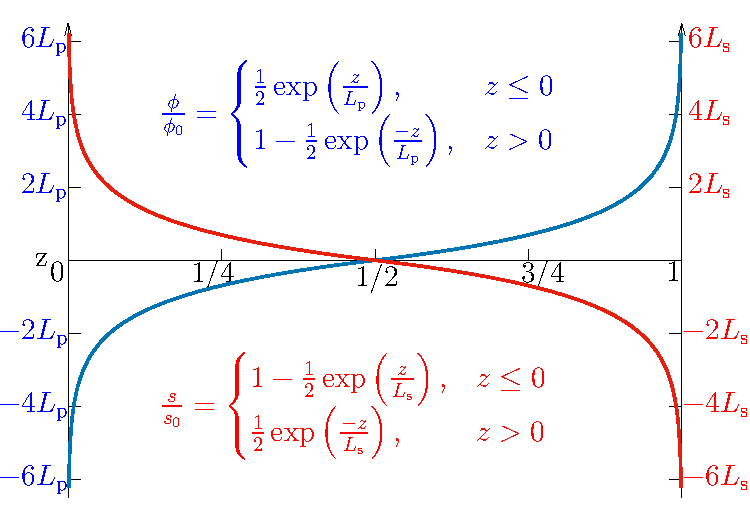
\includegraphics[width=0.3\paperwidth]{base_state.pdf}
          \end{figure}

          \vspace{-1cm}

          \centering \footnotesize Figure 3. Choice of base states for the
          particle and solute concentrations. The transitions have length scales
          $L_{\text{p}}$ and $L_{\text{s}}$ respectively.
          
      \end{block}

    \end{column}

    \begin{column}{0.6\paperwidth}
      \begin{block}{Non-dimensionalisation and generalised eigenvalue problem}
        \begin{columns}[t]
          \begin{column}{0.2\paperwidth}
            \centering We nondimensionalise the system using the characteristic length and velocity scales

            \vspace{-1cm}
            
            \begin{columns}[t]
              \begin{column}{0.11\paperwidth}
                \centering
                
                $$ L_{\text{c}} = L_{\text{p}} $$
                
              \end{column}
          
              \begin{column}{0.1\paperwidth}
                \centering

                $$ U_{\text{c}} = \frac{g L_{\text{p}}^{2}}{\nu} $$

              \end{column}

            \end{columns}

          \end{column}

          \begin{column}{0.3\paperwidth}
            \centering This gives seven dimensionless parameters

            \vspace{-1cm}
        
            $$ \Rey = \frac{g L_{\text{p}}^{3}}{\nu^{2}}, \quad  \quad U_{\text{p}}' = \frac{\nu U_{\text{p}}}{g L_{\text{p}}^{2}} \quad \quad L_{\text{s}}' = \frac{L_{\text{s}}}{L_{\text{p}}}$$

            \vspace{-1cm}
        
            $$A_{\beta} = \frac{\alpha s_{0} \nu^{2}}{g L_{\text{p}}^{3}}, \quad  \quad A_{\gamma} = \frac{\rho_{\text{p}} \nu^{2}}{g L_{\text{p}}^{3} \rho_{0}} \quad \quad \Sc_{\text{s}} = \frac{\nu}{D_{\text{s}}},  \quad  \quad \Sc_{\text{p}} = \frac{\nu}{D_{\text{p}}} $$

          \end{column}
        \end{columns}

        \vspace{1cm}

        Can express problem as a generalised eigenvalue equation
        
        $$ \begin{pmatrix}
          \frac{1}{\Rey}\left(\frac{\mathrm{d}^{4}}{\mathrm{d} z'^{4}} - 2 k'^{2} \frac{\mathrm{d}^{2}}{\mathrm{d} z'^{2}} + k'^{4}\right) &  k'^{2} A_{\beta} & k'^{2} A_{\gamma} \\[0.3em]
          \frac{\partial s^{(0)}}{\partial z'} & \frac{1}{\Rey \Sc_{\text{s}}} \left(k'^{2} - \frac{\mathrm{d}^{2}}{\mathrm{d} z'^{2}} \right) & 0 \\[0.3em]
          \frac{\partial \phi^{(0)}}{\partial z'} & 0 & \frac{1}{\Rey \Sc_{\text{p}}} \left(k'^{2} - \frac{\mathrm{d}^{2}}{\mathrm{d} z'^{2}} \right) - U_{\text{p}}' \frac{\mathrm{d}}{\mathrm{d} z'} 
        \end{pmatrix} \begin{pmatrix}
              \hat{u_{z}} \\[0.3em]
              \hat{s} \\[0.3em]
              \hat{\phi}
        \end{pmatrix} = i \omega \begin{pmatrix}
              \left(\frac{\mathrm{d}^{2}}{k'^{2} - \mathrm{d} z'^{2}}\right) &  \quad 0 \quad & \quad 0 \quad \\[0.3em]
              0 & 1 & 0 \\[0.3em]
              0 & 0 & 1
        \end{pmatrix} \begin{pmatrix}
              \hat{u_{z}} \\[0.3em]
              \hat{s} \\[0.3em]
              \hat{\phi}
        \end{pmatrix}$$

        \vspace{1cm}
        
        \centering This is a generalised eigenvalue problem and is solved for the eigenvalue $\omega = \Omega + i \sigma$. Solutions where $\sigma < 0$ are unstable, and the associated growth rate is $|\sigma|$. We can therefore predict the fastest growing perturbation wavelength $\lambda_{\text{max}} = 2 \pi / k_{\text{max}}$ which maximises $|\sigma|$ for different values of the dimensionless parameters. 
      \end{block}

    \end{column}

  \end{columns}

  \begin{block}{Special case: Rayleigh-Taylor instability}
    \begin{columns}[t]
      \begin{column}{0.3\paperwidth}
        \centering To validate the model, we consider the special case of a single phase ($s_{0} = 0$) in the absense of a settling velocity ($U_{\text{p}}' = 0$). This reduces the problem to that of the well studied Rayleigh-Taylor problem. 

        \begin{figure}
            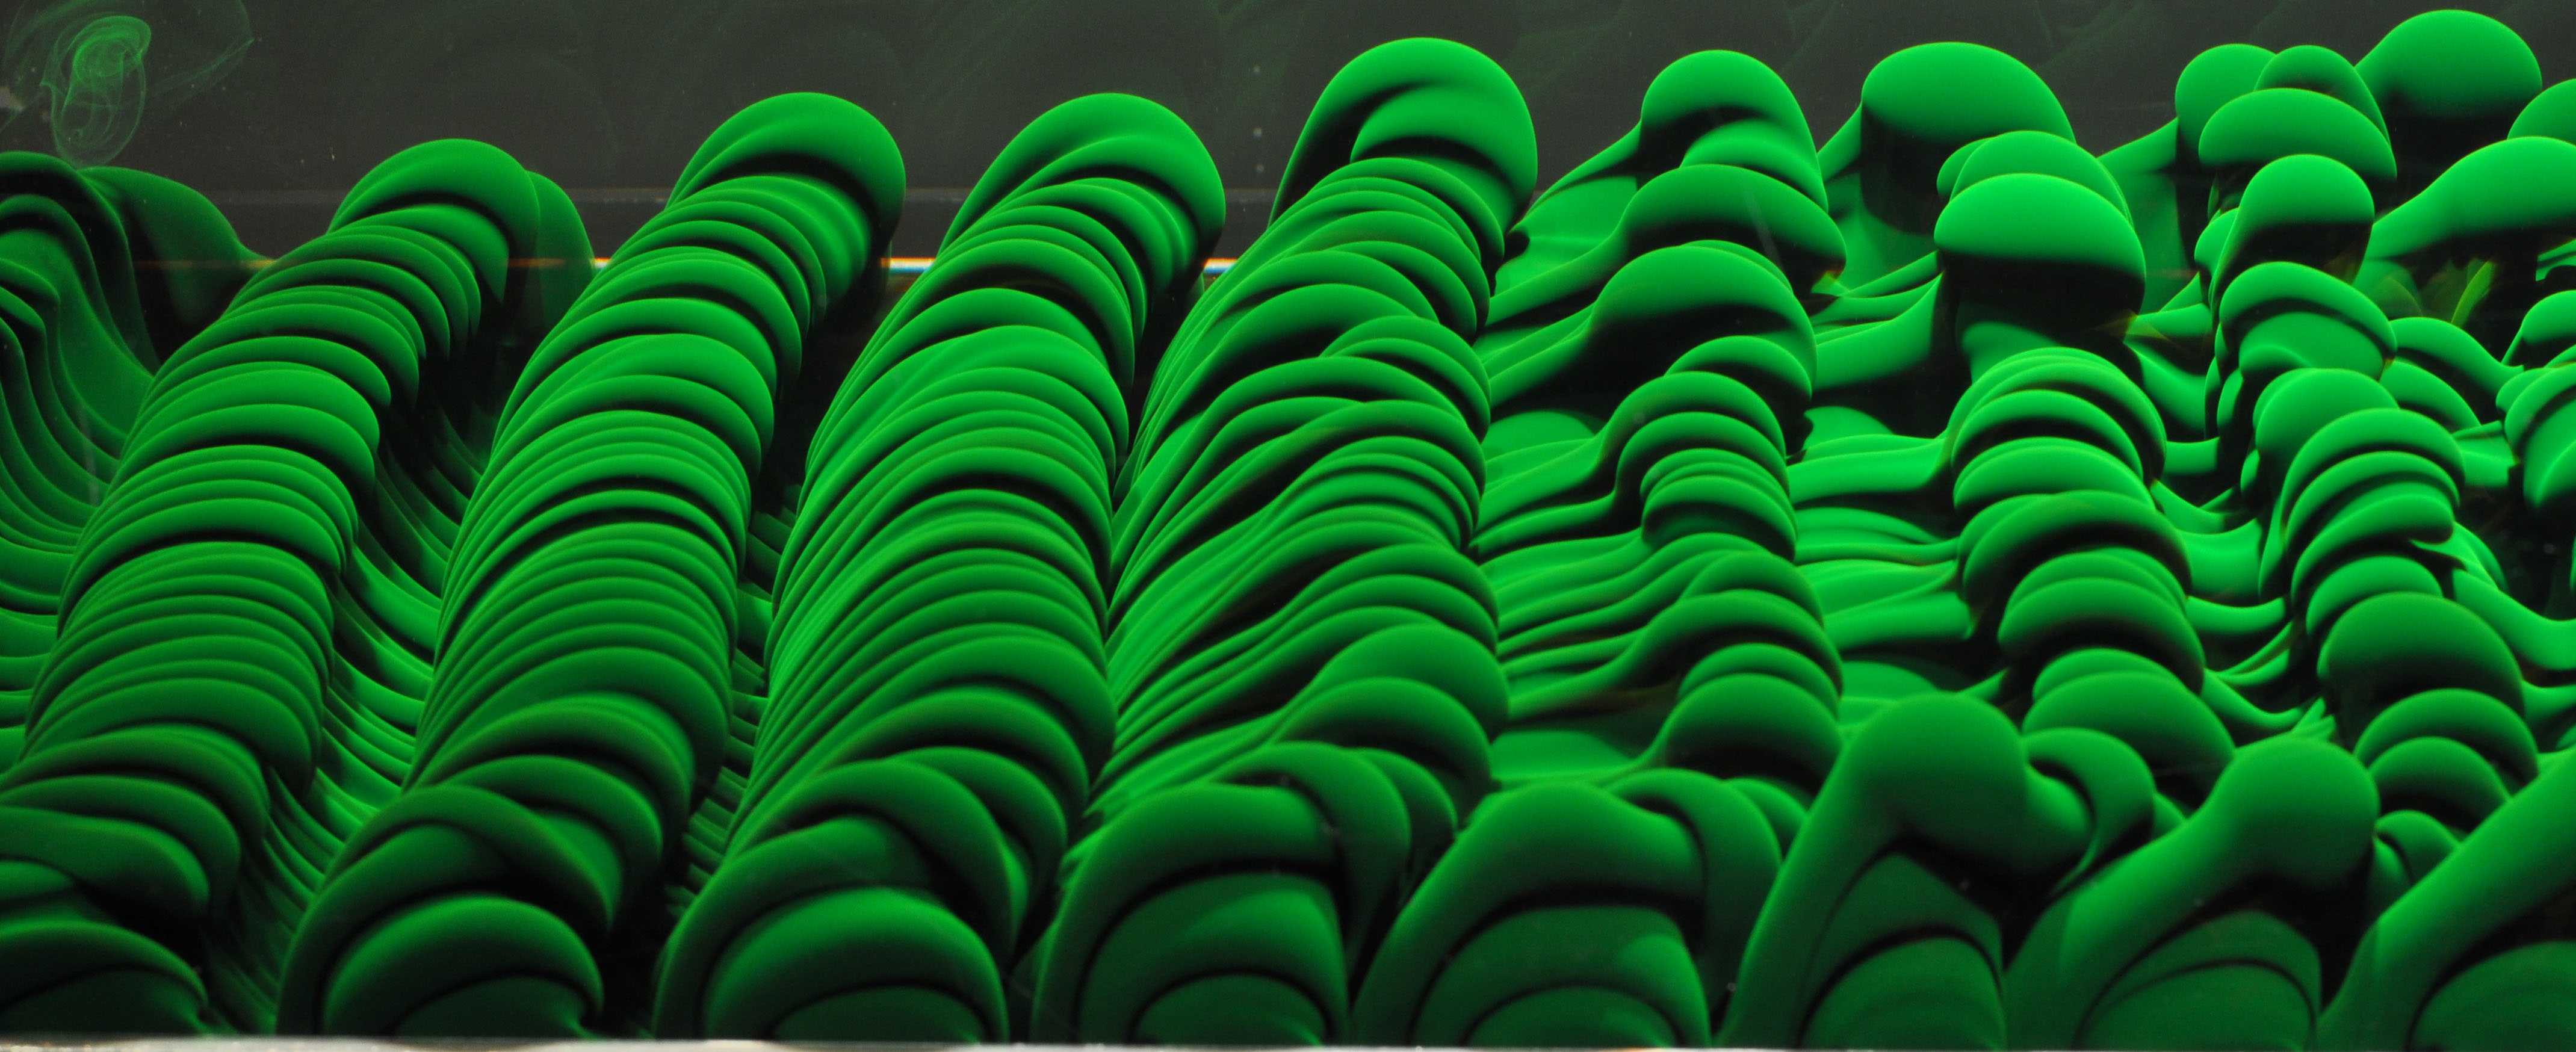
\includegraphics[width=0.3\paperwidth]{Megan.jpg}
        \end{figure}

        \vspace{-0.5cm}

        \centering \footnotesize Figure 4. Experimentally produced Rayleigh-Taylor instability. The green fluid is lighter than the overlying clear fluid. Credit: Megan Davies Wykes

        \vspace{0.5cm}

        \normalsize Choose sufficiently large $\Rey (10^{4})$ and $\Sc_{\text{p}} (10^{3})$ that system becomes independent of them \\
      \end{column}

      \begin{column}{0.3\paperwidth}

        \vspace{-0.5cm}

        \begin{figure}
          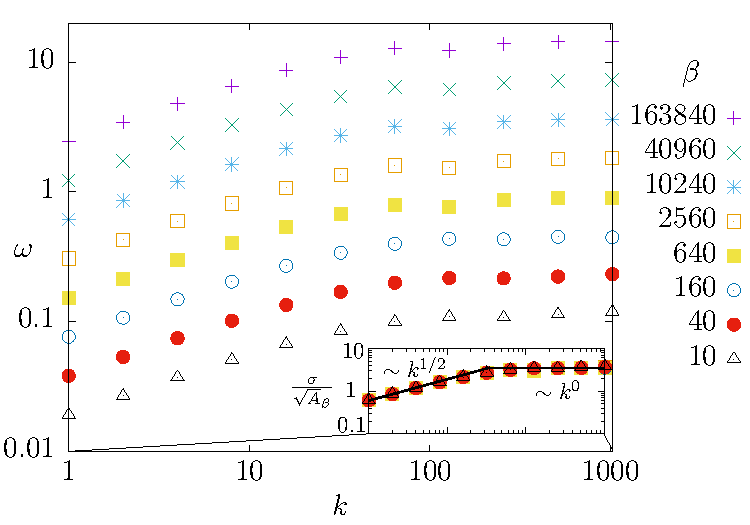
\includegraphics[width=0.3\paperwidth]{RT_dispersion.pdf}
        \end{figure}

        \vspace{-0.8cm}

        \centering \footnotesize Figure 5. Dispersion relation showing that $\sigma \sim A_{\gamma}$. There are two regimes of $k^{\prime}$ dependence, when $k^{\prime} < 1$, $\sigma \sim k^{\prime 1/2}$ and when $k^{\prime} > 1$, $\sigma \sim k^{\prime 0}$. 
      \end{column}

      \begin{column}{0.3\paperwidth}

        \vspace{1cm}
        
        \begin{columns}[c]
          
          \begin{column}{0.15\paperwidth}

            \centering $k^{\prime} < 1 \quad (\lambda > 2 \pi L_{\text{p}})$

          \end{column}

          \begin{column}{0.15\paperwidth}

            \centering $k^{\prime} > 1 \quad (\lambda < 2 \pi L_{\text{p}})$

          \end{column}
        \end{columns}

        \vspace{1cm}

        \begin{columns}[c]
          
          \begin{column}{0.15\paperwidth}

            \centering Wavelength is larger than the transition region. Scaling behaviour the same as for an infinitesimally thin transition zone. \\

          \end{column}

          \begin{column}{0.15\paperwidth}

            \centering Wavelength is shorter than the transition region. Growth rate independent of wavenumber. \\

          \end{column}
        \end{columns}

        \vspace{1cm}

        \begin{columns}[c]
          
          \begin{column}{0.15\paperwidth}

            \centering $$\omega \sim \left(\frac{g k \rho_{\text{p}}}{\rho_{0}}\right)^{1/2}$$
        
          \end{column}

          \begin{column}{0.15\paperwidth}

            \centering $$\omega \sim \left(\frac{g \rho_{\text{p}}}{L_{\text{p}} \rho_{0}}\right)^{1/2}$$

          \end{column}
        \end{columns}
      \end{column}

    \end{columns}
        
  \end{block}
\end{frame}
\end{document}

